\documentclass{article}


% if you need to pass options to natbib, use, e.g.:
%     \PassOptionsToPackage{numbers, compress}{natbib}
% before loading neurips_2022


% ready for submission
%\usepackage{neurips_2022}


% to compile a preprint version, e.g., for submission to arXiv, add add the
% [preprint] option:
%\usepackage[preprint]{neurips_2022}


% to compile a camera-ready version, add the [final] option, e.g.:
\usepackage[final]{neurips_2022}


% to avoid loading the natbib package, add option nonatbib:
%    \usepackage[nonatbib]{neurips_2022}


\usepackage[utf8]{inputenc} % allow utf-8 input
\usepackage[T1]{fontenc}    % use 8-bit T1 fonts
\usepackage{hyperref}       % hyperlinks
\usepackage{url}            % simple URL typesetting
\usepackage{booktabs}       % professional-quality tables
\usepackage{amsfonts}       % blackboard math symbols
\usepackage{nicefrac}       % compact symbols for 1/2, etc.
\usepackage{microtype}      % microtypography
\usepackage{xcolor}         % colors
\usepackage{graphicx}
\usepackage{subfig}

\title{Stroke Prediction Model}


% The \author macro works with any number of authors. There are two commands
% used to separate the names and addresses of multiple authors: \And and \AND.
%
% Using \And between authors leaves it to LaTeX to determine where to break the
% lines. Using \AND forces a line break at that point. So, if LaTeX puts 3 of 4
% authors names on the first line, and the last on the second line, try using
% \AND instead of \And before the third author name.


\author{%
  Majd Owda \\
  AI engineering\\
  Bahcesehir University\\
  Turkey, Istanbul \\
  \texttt{majd.owda@bahcesehir.edu.tr,} \\
  \And 
  Yaman Alomar \\
  AI engineering\\
  Bahcesehir University\\
  Turkey, Istanbul \\
  \texttt{yaman.alomar@bahcesehir.edu.tr} \\
  \And 
  Anas Alyafeai \\
  AI engineering\\
  Bahcesehir University\\
  Turkey, Istanbul \\
   \texttt{anas.alyafei@bahcesehir.edu.tr} \\
  }
  % examples of more authors
  % \And
  % Coauthor \\
  % Affiliation \\
  % Address \\
  % \texttt{email} \\
  % \AND
  % Coauthor \\
  % Affiliation \\
  % Address \\
  % \texttt{email} \\
  % \And
  % Coauthor \\
  % Affiliation \\
  % Address \\
  % \texttt{email} \\
  % \And
  % Coauthor \\
  % Affiliation \\
  % Address \\
  % \texttt{email} \\



\begin{document}


\maketitle


\begin{abstract}
  A machine learning model that predicts weather a person will have a stroke or not based on lifestyle features such as bmi, age ,hypertension and many other features using the powerful gradient boosting algorithm(XGBoost).
\end{abstract}


\section{Introduction}
a boosting gradient algorithm(XGBoost) was used in a machine learning model to predict weather a person will have a stroke or not based on lifestyle features where it was needed to deal with some missing data and needed to be cleaned.  
various kind of approaches were used in order to reach the desired accuracy.




\section{Description of the data}


The dataset used is a combination between real world data, and a synthetic data which is generated by a deep learning model trained on the real world data, the dataset consists of 20410 rows and 12 columns, the categorical features consists of,  “Gender, Heart Disease, Hypertension, Ever Married, Work Type, Residence Type, Smoking Status”, whilst the numerical features are, “Age, BMI, Avg Glucose Level”,  the “Stroke” is the target, while the “id” is a unique identifier. Also all the columns are the same for the test data, and you have to predict the probability of having a “Stroke”.

\section{Description of methods}
In this model we used a variation of methods and approaches until we reached the desired accuracy of prediction, and they list as the following:

\subsection{Data Understanding}
In this part we did the appropriate approaches to understand the data, so it can be easier to manipulate it and to decide which model could be used.

\subsection{Reading the data and merging it}
First, we merged the datasets that we are going to use, and we dropped the duplicates.

\subsection{Understanding the data}
Here we started analyzing the data in order to understand it by listing the description and a summary about the data. Then we filled the missed data in the “BMI” column, we did it by taking the median, because we had an outliers after the 3’rd quantile.



\subsection{Visualizing the data}
We did different visualizations for the data, First, we started by doing a Pie Chart to know which percentage of the data has a “Stroke”. Then, we did Scatter Plots for the numerical features and the age with a Hue for every categorical feature, for both the train and test sets. Next, a Bar Plots were done to know the proportions for every categorical feature for both the train and test set, and the likelihood of having a stroke for every proportion. After that, KDE Plots for both the train and test sets, a Histogram Plots with a hue for the stroke, and Box Plots, which was done for every numerical feature we have. Finally, we did normal Histogram Plots for every numerical feature to check the normality of our data.

\section{Data preparation and preprocessing}
In this part we did the Feature engineering, encoding and scaling for the data so it can be utilized by the model.

\subsection{Feature engineering}
New feature was introduced by doing some operations on the original data, the new feature was called "risk factors", we applied 5 conditions and if it meets the conditions it will be 1 and if it does not then it is 0.so in summary, we  calculated a risk factor score based on specific conditions related to the individual's health attributes such as glucose level, age, BMI, hypertension, heart disease, and smoking status.

\subsection{Encoding and scaling}
Encoding was done by “OneHotEncoder”, from “feature.engine” library, for the categorical features. And scaling was done by “SklearnTransformerWrapper”, from “feature.engine” library, and “StandardScaler” from “sklearn” library, for the numerical features. But unfortunately, this affected our score accuracy negatively, so in the final code, we did a simple encoding by hand, by mapping a new numerical values for every categorical feature, and no scaling was done for the numerical features.

\section{Modeling and Generating Predictions}
A bunch of models were used in our project and the one with best accuracy was chosen after evaluating every model.

\subsection{Logistic regression}
Our logistic regression is from “sklearn” library. First, we split the data using “train test split”. Then we encoded and scaled the data. Next, we applied the logistic regression on the train dataset, and we found the accuracy by using a confusion matrix. Finally, we applied the model on the test dataset and produced the predictions in “CSV” form.

\subsection{XGB Classifier}
we got the XGB classifier from the “xgboost” library. Firstly, we defined the parameters for the xgb classifier model and used various hyperparameters such as
1-max depth: this parameter controls the maximum depth of each tree in the boosting process and if we set higher the model will be more complex which might overfit the data.
2-eta: it is the learning rate; it determines the step size during each boosting iteration.
3- subsample: specifies the fraction of the training
instances to be randomly sampled for each tree.
4-Colsample bytree: It determines the fraction of features (columns) to be randomly sampled for each tree.
5- min child weight: This parameter defines the minimum sum of instance weight (hessian) needed in a child. Helps in preventing overfitting.
We also used other parameters such as gamma, lambda, alpha, max delta step, objective and eval metric. Next, we split the data using “train test split” and applied the XGB classifier on the train data and evaluated the model by using Confusion matrix. At the end, we used the model on the test dataset and generated the predictions and saved them to a “CSV” file.

\subsection{Other model that were used}
1-Random Forest Classifier 
\newline 2-LGBM Classifier
\newline 3-CatBoost Classifier
\newline

\begin{figure}[!htb]
  \centering
  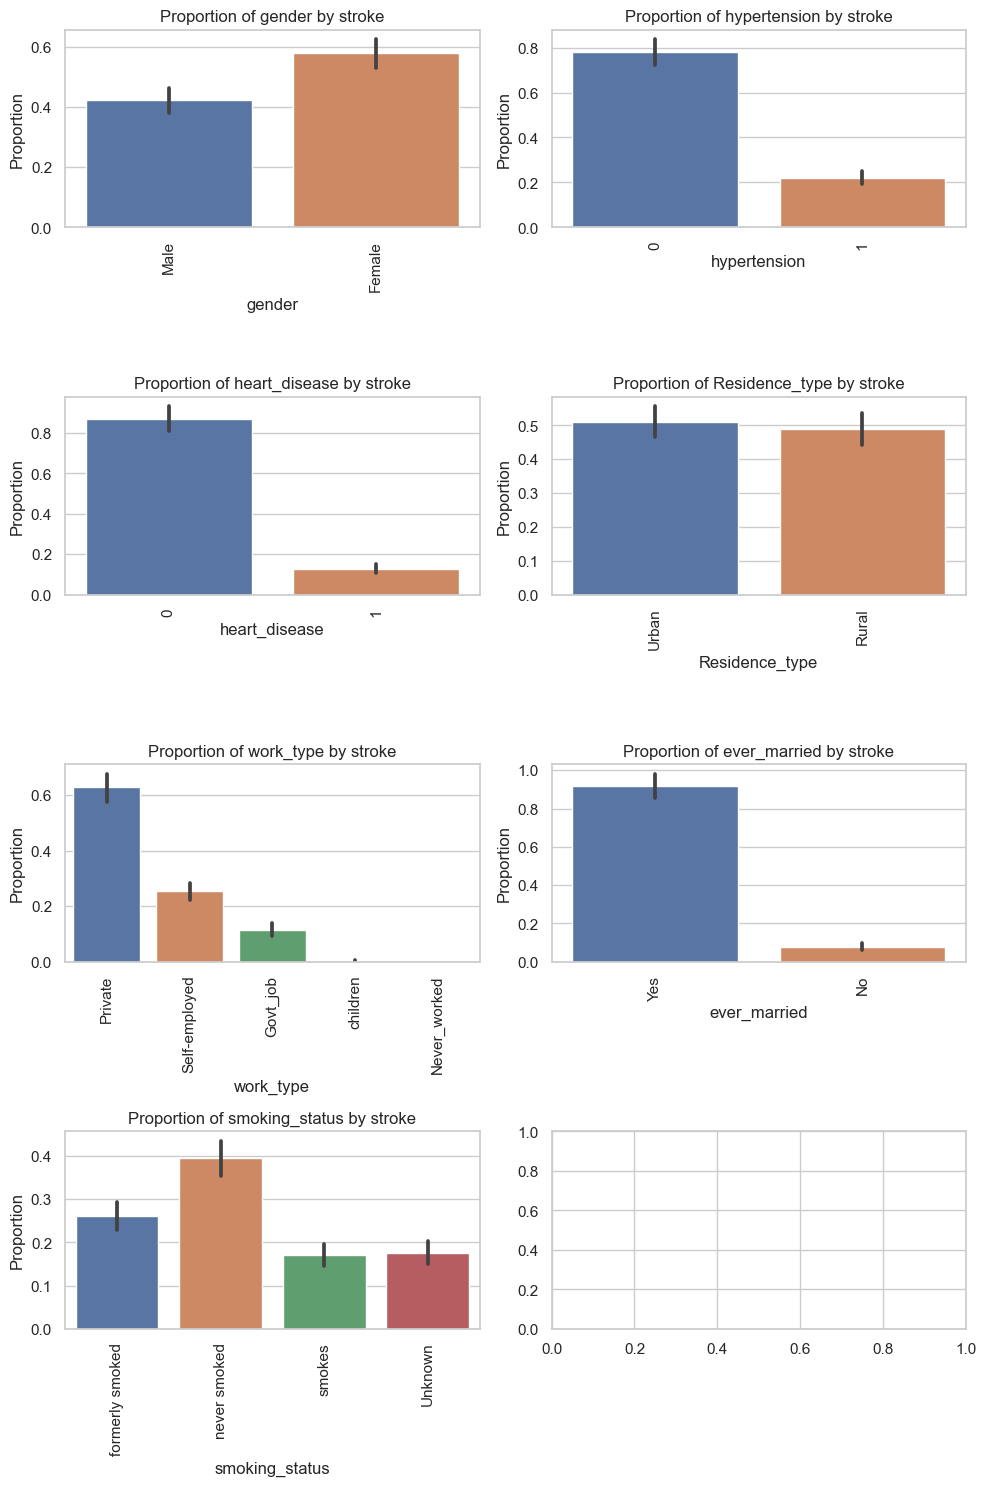
\includegraphics[width =150 ,height =150]{output.png}
  \caption{Proportions}
  \label{Proportions}
\minipage{0.32\textwidth}
  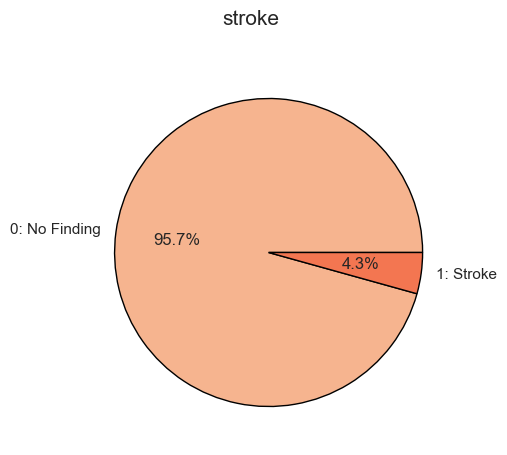
\includegraphics[width=\linewidth,height = 150]{stroke percantage.png}
  \caption{Stroke Percentage}\label{Pie}
\endminipage\hfill
\minipage{0.32\textwidth}%
  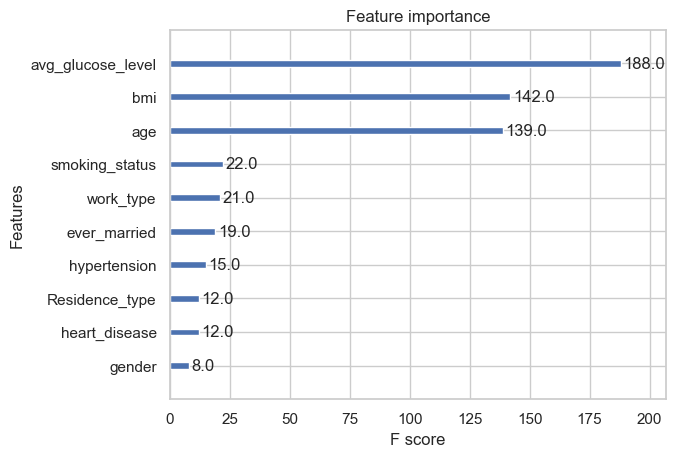
\includegraphics[width=\linewidth,height = 150]{FeatureImportance.png}
  \caption{Feature Importance}\label{F}
\endminipage
\end{figure}

%\begin{figure}[h]
  
  %\fbox{\rule[-.5cm]{0cm}{4cm} \rule[-.5cm]{4cm}{0cm}}
 % 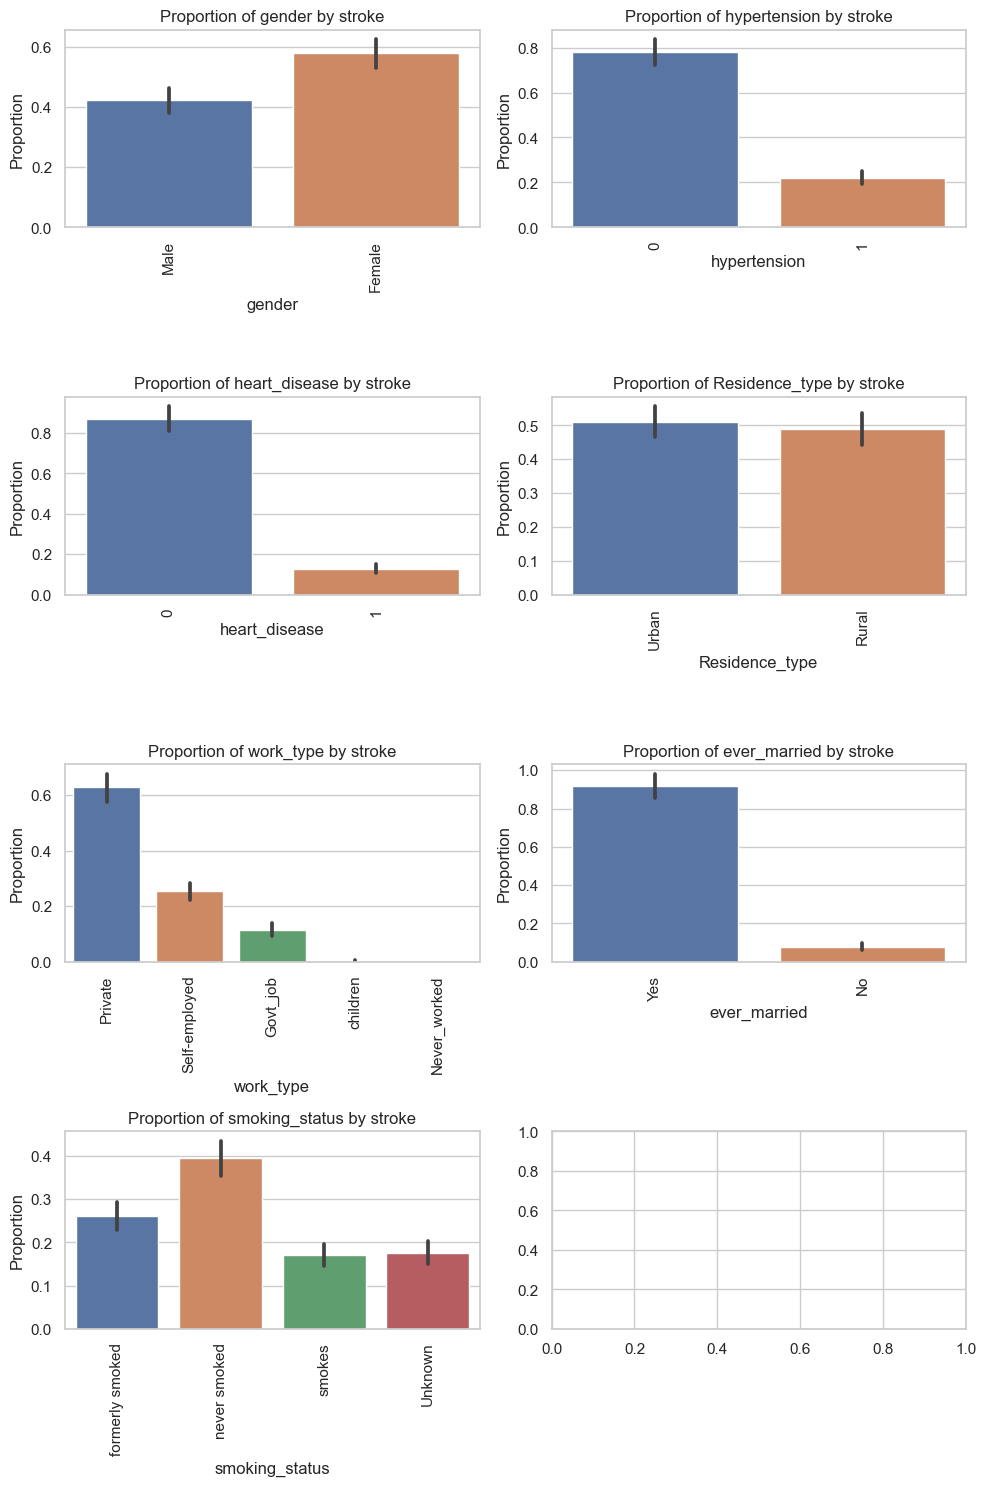
\includegraphics[width=0.3 \textwidth,left]{output.png}
  %\caption{Proportions}
  
%\end{figure}
  %\begin{figure}[h]
  %\centering
  %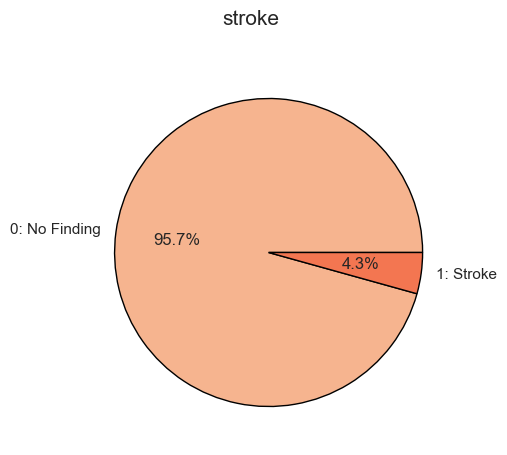
\includegraphics[width =150]{stroke percantage.png}
  %\caption{Stroke percentage}
  
%\end{figure}

%\begin{figure}[h]
 % \centering
%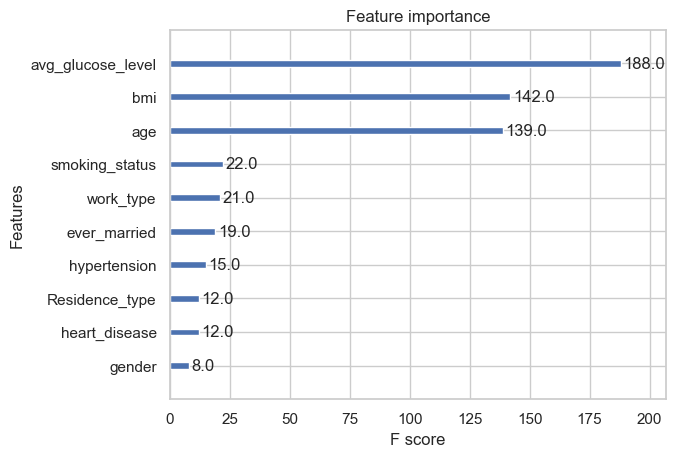
\includegraphics[width= 150]{FeatureImportance.png}
%\caption{Feature importance}
%\end{figure}
\section{summary of results}
As shown in Figure \ref{Pie} we can realize that the people who have a “Stroke” holds a 4.3\% of the dataset, while people who don’t have a “Stroke” are 95.7\%. In Figure \ref{Proportions} proportions graph we can see what the proportion of each value for each feature is. And as can be seen in \ref{F} feature importance graph shows which features are the most effective on the algorithm.
By analyzing the graphs we can realize that the dataset is somewhat biased, because the “Stroke” holds only a small percentage of the dataset, and some features values are not logical, such as the “hypertension”, “heart disease” and “smoking status”, as we can clearly see in our dataset the people who don’t have a “heart disease”,  “hypertension” and don’t hold the biggest proportion of having a “stroke”.  The model also depends on the numerical features more than the categorical, while in real world “hypertension” and “smoking status” are main causes of having a stroke. And this is maybe happening because a big part of the data was generated using AI.
After evaluating various models, we realized that scaling and encoding the data affected the score negatively while working with some models, while the “XGBClassifier” had a score of (0.90201) without scaling and encoding. The score went down to (0.89879) after. On the other hand, “Logistic Regression” had a better score with scaling and encoding. Because of the bias in the data the “Feature Engineering” wasn’t also a good idea, where introducing new features affected the model negatively.

\begin{table}[h]
  \caption{Scores of the models}
  \label{sample-table}
  \centering
  \begin{tabular}{ll}
    \toprule
    Model & Score \\
    \midrule
    Logistic regression & 0.89224 \\
    LGBM & 0.89914\\
    CatBoost & 0.89524 \\
    Random forest classifier & 0.88853 \\
    XGBoost classifier & 0.90201 \\
    \bottomrule
  \end{tabular}
\end{table}

\section{Discussion}
why did encoding and scaling affect the accuracy of our model negatively? 
\newline "OneHotEncoder" changes the categorical variables to numerical variables and creates dummy variables, which can cause an inefficiency in tree based models such as "RandomForestClassifier" and "XGB Classifier". On the other hand, Encoding is advantageous for logistic regression by preserve the relationships within the data , "OneHotEncoder" ensures that the model captures the correct relationships and avoids arbitrary assumptions.
\newline
The reason why "Logistic Regression" performs better with scaling is because it helps to ensure that features with different scales do not dominate the learning process and because it makes the features magnitudes and directions more comparable. Scaling is not a critical preprocessing method and that is maybe why it did not have a big impact on the other models weather it was done or not.



\section{Roles contribution}
Our group made significant contributions throughout the project, ensuring its success.No one in our group had a specific role as we all gave our different ideas about every step that we were required to do in the project and then we implemented the best approach and went with it. Overall, everyone did their job and gave it their best.

\section{Links}
[github] https://github.com/YamanAlo/Stroke-Prediction-model
\newline
[Deployment] https://huggingface.co/spaces/MajdOD/gradio-Stroke-prediction

\subsection{References}
[1] https://www.kaggle.com/code/k0takahashi/ps-s3e2-2023-stroke-prediction-8th-place
\newline
[2] https://www.cdc.gov/stroke/about.htm#:~:text=A\%20stroke\%2C\%20sometimes\%20called\%20a,term\%20disability\%2C\%20or\%20even\%20death.


\end{document}
